In this chapter, we present preliminary surface stress and adhesion energy data collected for two types of silicone with various stiffnesses. We first used Gelest brand silicone to obtain our preliminary data and tune the operation of our device. We then switched to Dow-Corning brand silicone to continue more extensive measurements. First we give a brief background of the materials used. 


\section{Organosilicon Polymer Chemistry}
\label{section:polychem}
PDMS, or Polydimethylsiloxane, is a commonly used polymer gel in the field of soft condensed matter. The gel is composed of a polymer network connected by crosslinkers, with additional free polymer in the fluid phase. When stretched, the large number of covalent bonds resist deformation on a macroscopic level.\footnote{PDMS consists of covalent crosslinkers, however, many compliant materials are a result of physical crosslinkers (e.g. gelatin). When physical crosslinkers are stretched, the configuration of the system changes such that the tangled crosslinkers begin to unwind and untangle. From a statistical mechanics perspective, this decreases the configurational entropy, thus increasing the free energy \cite{Andreotti2020}.} 

%physical crosslinkers: add to ch1 brief descriptions.
%When stretched, the configuration of the system changes such that the tangled crosslinkers begin to unwind and untangle. From a statistical mechanics perspective, this decreases the configurational entropy, thus increasing the free energy. 

Below (Fig. \ref{fig:DMS-V31}) is the chemical structure for the vinyl-terminated PDMS (Gelest) that comprises the Gelest silicone. Dow-Corning is also a PDMS, but has an undisclosed molecular composition.
% Set chemical bonds length
\setatomsep{20pt}

% -------------From chemfig manual, useful macro--------------------
\newcommand\setpolymerdelim[2]{\def\delimleft{#1}\def\delimright{#2}}
\def\makebraces(#1,#2)#3#4#5{%
	\edef\delimhalfdim{\the\dimexpr(#1+#2)/2}%
	\edef\delimvshift{\the\dimexpr(#1-#2)/2}%
	\chemmove{
		\node[at=(#4),yshift=(\delimvshift)]
		{$
			\left\delimleft
			\vrule height\delimhalfdim depth\delimhalfdim width0pt
			\right.
			$};
		\node[at=(#5),yshift=(\delimvshift)]
		{$
			\left.
			\vrule height\delimhalfdim depth\delimhalfdim width0pt
			\right\delimright_{\rlap{#3}}
			$};
	}%
}

%PDMS DMS-V31 Figure
\begin{figure}[h!]
	\centering
	\scalebox{1.75}{
		\setpolymerdelim()
		
		\chemfig{H_2C=C(-[-3]H)--[@{op,0}]Si(-[2]CH_3)(-[6]CH_3)-O--[@{cl,0}]Si(-[2]CH_3)(-[6]CH_3)-C(-[7]H)=CH_2}
		
		\makebraces(20pt,20pt){$\!\!n$}{op}{cl}
	}
	\label{fig:DMS-V31}
	\caption[DMS-V31]{Divinyl-terminated Polydimethylsiloxane (DMS-V31)}
\end{figure}
\noindent For Gelest, the crosslinker of the system is a trimethylsiloxane terminated 25--35\% methylhydrosiloxane - dimethylsiloxane copolymer (Gelest HMS-301). The crosslinker is much shorter on average than the PDMS, containing roughly 20--30 repeating monomer groups. The single hydrogen on the methylhydrosiloxane is weakly bound and can be replaced by one of the hydrogen atoms in the PDMS. This bonding happens repeatedly, creating long twisted chains which comprise the mesh network of the gel. Increasing the density of crosslinkers provides an easy and controllable method to vary the gel's stiffness \cite{Andreotti2020}. 

%PDMS Crosslinker HMS-301 Figure
\begin{figure}
	\centering
	\scalebox{1.75}{
		\setpolymerdelim()
		%the [@{op,offset}] and [@{cl,offset}] are for the giant parentheses macro function.
		\chemfig{H_3C-Si(-[2]CH_3)(-[6]CH_3)-O--[@{op,0}]Si(-[2]H)(-[6]CH_3)-O-[@{cl,.5}]-[@{op2,.5}]Si(-[2]CH_3)(-[6]CH3)-O--[@{cl2,0}]Si(-[2]CH_3)(-[6]CH_3)-CH_3}
		
		\makebraces(20pt,20pt){$\!\!m$}{op}{cl}
		\makebraces(20pt,20pt){$\!\!n$}{op2}{cl2}
	}		
	\label{fig:HMS-301}
	\caption[HMS-301]{Trimethylsiloxane terminated 25-35\% methylhydrosiloxane ($m$) -- dimethylsiloxane ($n$). This is the crosslinker for Gelest silicone (HMS-301).}
\end{figure}

\begin{table}[h!]
	\begin{center}
		\setstretch{1.25}
		\begin{tabular}{|c||c||c|}
			\hline
			Mix Ratio (A:B) & Young's Modulus (kPa) & Sol Fraction (\%)\\
			\hline
			$7.5:1$ & $2.5 \,\pm\, 0.1$ & 65.2\\
			\hline
			$9:1$ & $5.0 \, \pm\, 0.1$  & 64.7\\
			\hline
			$11:1$ & $10.0 \,\pm\, 1$  & 63.7\\
			\hline
		\end{tabular}
	\end{center}
	\label{tab:recipes}
	\caption[PDMS ratios Characterization]{PDMS gel characterization for Gelest silicone. By varying the relative density of the crosslinkers, one can predictably control the stiffness of the gel.}
\end{table}




\subsection{Silicone Preparation and Spin-Coating}
Before spin-coating it is useful to coat the base with fluorescent beads to help determine the substrate's thickness. The sole purpuse of this coating is to help locate the substrate's bottom surface, so a dense bead coverage is not required and could potentially be harmful if there is significant light bleeding\footnote{When the light from the fluorophores is intense enough, they are detected in the adjacent images in the vertical stack. This phenomenon is referred to as ``light bleeding.''}. To coat the base, we pipet 40~nm fluorescent beads onto the glass of PDMS and let sit for 30--60 seconds. Full directions for preparing a fluorescent bead solution can be found in Appendix B. After this time, we return the fluorescent beads back to the solution for re-use. A significant number of beads will remain on the base, however. To remove some excess, we gently wash the substrate with de-ionized water. For a glass coverslip, we simply submerge the entire slip in water and gently remove it at a 45\degree ~angle, using surface tension to prevent the water from breaking up into smaller droplets. This process is slightly more difficult for the petri dish due to the larger size. We have had success using 1000~mL beaker tilted at an angle, though any container with a large enough opening may substitute. It is also possible to use an autopipet for washing by simply repeating the same process used for the fluorescent bead coating, only with water instead this time. We have had mixed success with this technique, however; it leaves a water droplet on the surface and often creates an uneven coating of fluorescent beads, manifested as fluorescent streaks across the surface.

After the first layer of fluorescent beads is coated, it is time to spin-coat the soft substrate. We aim to make our spin-coated substrates around  80--100~$\mu$m thick. Depending on the silicone, we wait a different amount of time before spin-coating onto the prepared base. This allows the curing process to increase the silicone's viscosity enough to remain on the base when spun. As an extreme example, consider trying to spin-coat water; it would all fling off the base. We coat our substrate onto coverslips for ``zero applied strain'' data or on PDMS sheets from SMI (Shore Durometer: 40, Thickness: 0.005'') for stretching data. Gelest 9:1 cures rapidly at room temperature, so no waiting time necessary. For Dow Corning 1:1, we wait 45--60 minutes after combining parts A and B before spin-coating.

To help with the evenness of the coating, we degas the gel by leaving it in a vacuum chamber for a few minutes. A few small bubbles are not of concern, as the process of transferring the gel to the base is enough to pop any remaining stragglers. We have found that a ``glob'' of gel roughly half the diameter of the base spin-coated at 500 rpm for 40 seconds is enough to create an even coating of roughly 100 $\mu$m for both Gelest 9:1 and Dow-Corning 1:1 PDMS.

Coating a coverslip with silicone is a straightfoward process where hardly anything can go wrong. Coating the stretchable PDMS base, however, requires some creativity to find the steps necessary to return the best results. We cut the SMI PDMS sheet with an X-acto knife and use a standard Petri dish (3.5'' diameter) as a template. In order to avoid snagging, we cut out the disk before removing the paper sheets on both sides of the silicone and tape the Petri dish to the paper to help prevent the dish from slipping while cutting. Unlike the glass coverslip, the PDMS base is not rigid and must be placed on a firm surface, such as a Petri dish, for spin coating. This leaves the possibility for air bubbles to become trapped in between the PDMS and Petri dish interface, a surefire way to produce an unevenly coated substrate. To avoid this, we remove the top paper sheet from the newly cut PDMS, then place the Petri dish on the exposed silicone. This creates a Petri dish with a silicone disk on top and a paper sheet on top of that. We then remove the air bubbles by pressing on the silicone sheet from the center outwards. Finally, any tiny, remaining air bubbles can hopefully be removed by placing the Petri dish in a vacuum chamber for a few minutes. It is at this point that we coat the PDMS with fluorescent beads and wash (as described early) before placing the petri dish onto the spin-coater and proceeding as described above.

After spin-coating, the silicone requires time to cure. We cure Dow-Corning 1:1  at room temperature for at least 24 hours. For Gelest 9:1, we oven cure at $70 \degree$ C for at least 24 hours. Either silicone can be cured at room temperature or in the oven so long as a sufficient amount of time is waited, however, we have used these curing parameters to maintain consistency and parallel the techniques used in previous literature \cite{xu2017direct}.

After the silicone cures, we coat the surface with fluorescent beads again. For the 40~nm bead solution prescribed in Appendix B, we allow the solution to soak for up to 1.5 minutes before removing and washing the substrate. While the fluorescent beads chosen are most susceptible to light at 440 nm, there is still the risk of photo-bleaching\footnote{When too much light is exposed to the fluorophores, a photochemical alteration causes them to no longer be able to fluoresce.} the fluorophores, and it is worth dimming the lab lights when working with them. 

\section{Preliminary Data: Gelest}
Because the 2017 measurement \cite{xu2017direct} (See Figure \ref{fig:2017natcomfig}) was obtained using Dow-Corning PDMS, our intention from the start was to use this material in our adhesion based measurements. However, due to technical difficulties\footnote{The Dow-Corning silicone was back-ordered.} we decided to use Gelest instead while we calibrated the process. In this chapter, we present these preliminary data because it shows that the surface stress for the substrate is increasing with strain.  

\subsection{Standard Candles}
Not only do we measure the depth and radii for a range of spheres, but we also measure a select few spheres at every strain. This allows us to track how any given sphere is changing---increasing our confidence that the shift in $\Upsilon$ and $ W $ is not just an artifact of noise---as well as provide a more palpable piece of evidence than just a comparison of averages. Below (Fig. \ref{fig:sc1unstretchedv8ml}) is the side profile for Gelest 9:1 ($\text{E}=6.3$ kPa). Notice how the indentation profile shifts upwards (less deep) to be flattened when the substrate is stretched. This shift is expected if the surface stress is increasing (see equation \ref{THEeqn}).

\begin{figure}[h!]
	\centering
	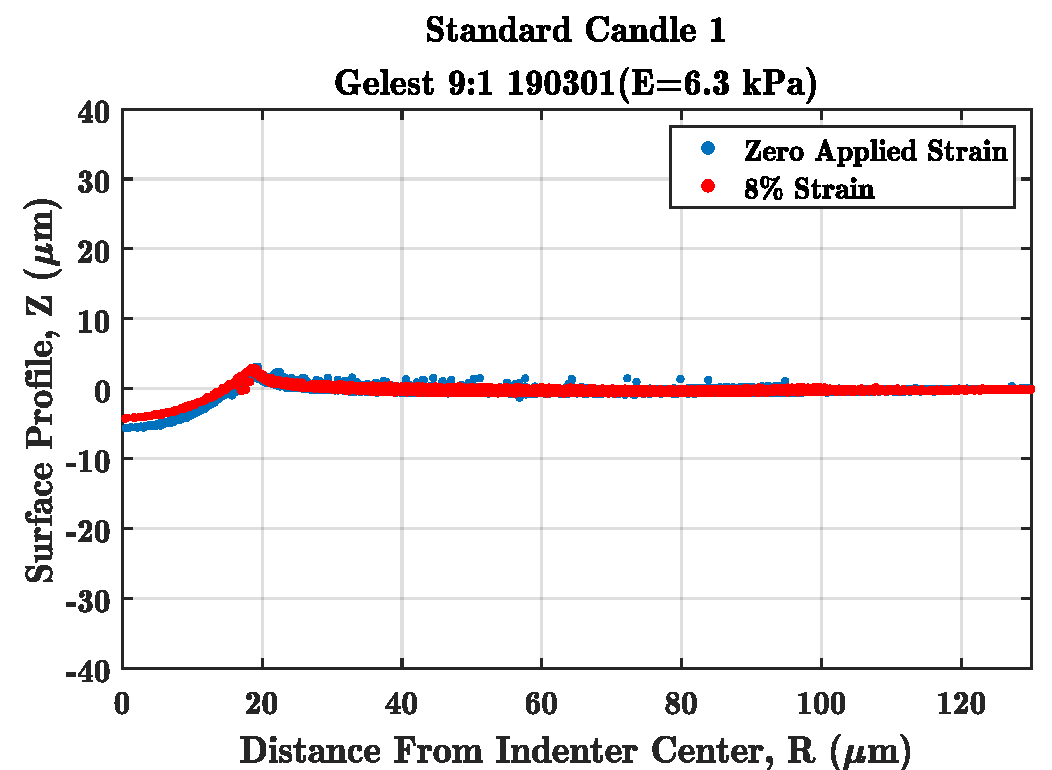
\includegraphics[width=\linewidth]{Chapters/Figures/stretch_v_unstretched_0-88-ST1}
	\caption[Side Profile Comparison: 8\%]{The side profile of the same sphere before and after stretch. Notice how after stretching, the sphere's indentation into the substrate is shallower.}	
	\label{fig:sc1unstretchedv8ml}
\end{figure}
\begin{figure}
	\centering
	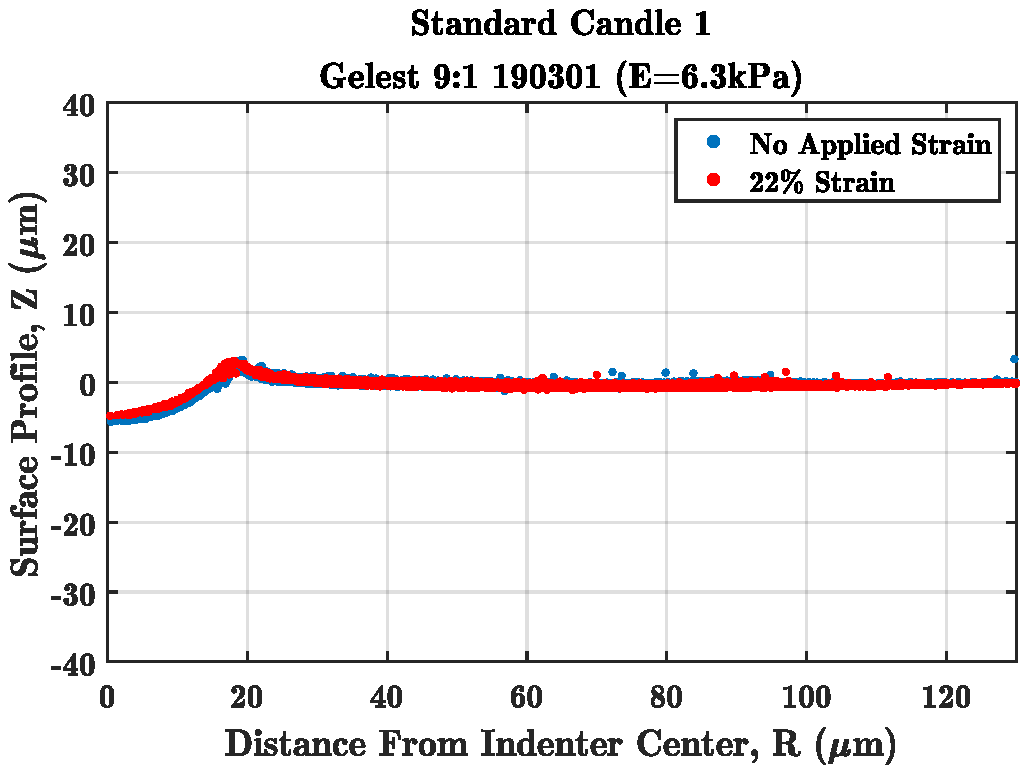
\includegraphics[width=\linewidth]{Chapters/Figures/stretch_v_unstretched_0-22-ST1}
	\caption[Side Profile Comparison: 22\%]{The side profile of the same sphere as in Figure \ref{fig:sc1unstretchedv8ml} before and after stretch at 22\% strain. Notice how after stretching, the sphere's indentation into the substrate is shallower.}
	\label{fig:stretchvunstretched0-22-st1}
\end{figure}

\begin{figure}[h!]
	\centering
	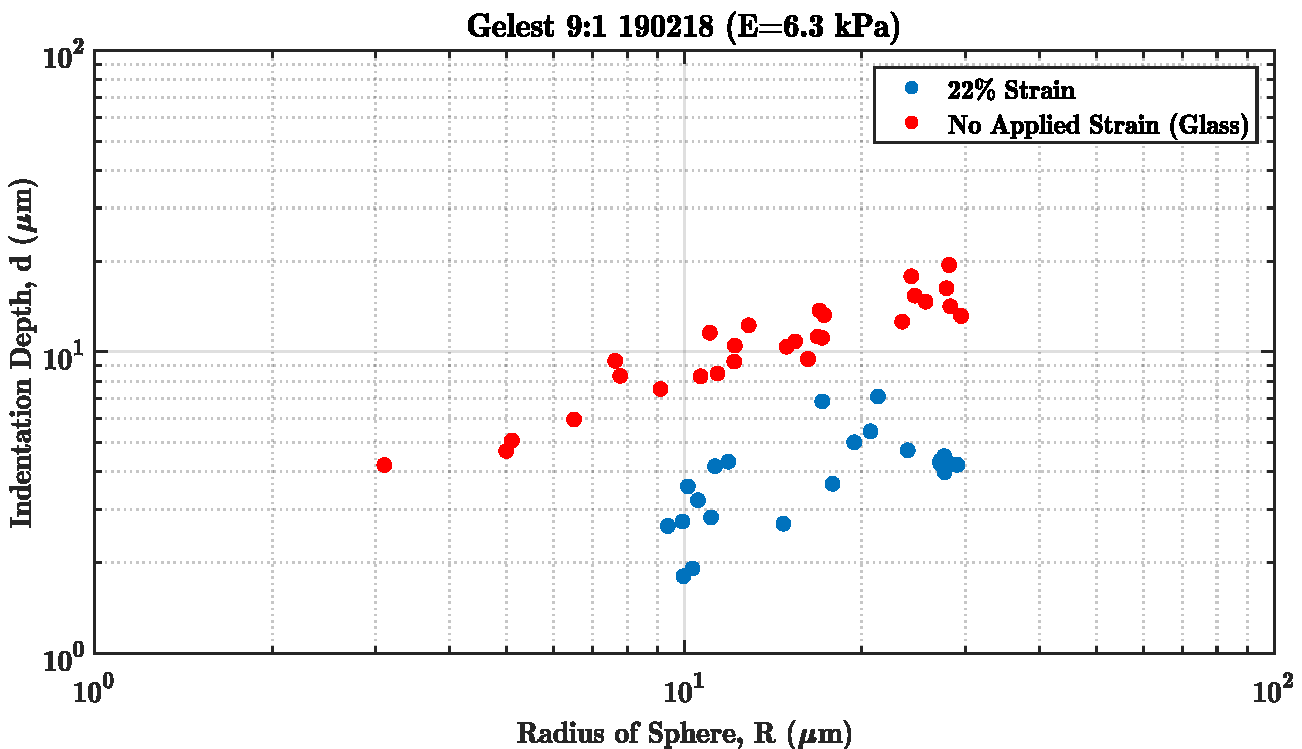
\includegraphics[width=\linewidth]{Chapters/Figures/g190218_glass_vs_22percent_dvsR.pdf}
	\caption[Glass vs. Stretched d vs. R]{For Gelest 9:1, the silicone under strain (blue) on average sinks less deep into the silicone than for the same silicone sample spun on glass (zero applied strain). The large noise for the strain-data means we can not meaningfully determine $ \Upsilon $ and $ W $ to measure the variation in $ \Upsilon(\epsilon)$ and $W(\epsilon)$.}
	\label{fig:glassvsstretched190218}
\end{figure}

The $ d $ vs.~$R$ data collected with substrates on our stretching apparatus have a lot of noise. As seen in Figure \ref{fig:glassvsstretched190218}, the $ d $ vs.~$R$ data collected on glass is far cleaner than that collected on the stretcher when strained. We can see the trend that under strain, the spheres sink into the substrate less deeply. At 22\% strain, we expect zero strain-stiffening of our elastic substrate, and conclude that this change in depth is a result of an increase of surface stress, $ \Upsilon $. Unfortunately, the $ d $ vs.~$R$ values are too noisy/scattered to make a reasonable fit to extract $ W $ and $ \Upsilon $ values.

The collapsed side profiles for spheres on a stretched substrate (see Figures \ref{fig:sc1unstretchedv8ml} and \ref{fig:stretchvunstretched0-22-st1}) do not ``collapse'' as cleanly as those for spheres on glass; one glass, the spread in fluorescent beads is narrower than for stretchable substrates. Furthermore, the side profiles are often tilted away from the surface profile, and require manual editing to correct the far field height. It is much more difficult, however, to adjust the tilt. This is further discussed in Section \ref{sec:DataConclusions}, and can be seen in Figure \ref{fig:190218gtiltedaxisexample}.   

\begin{figure}[h!]
	\centering
	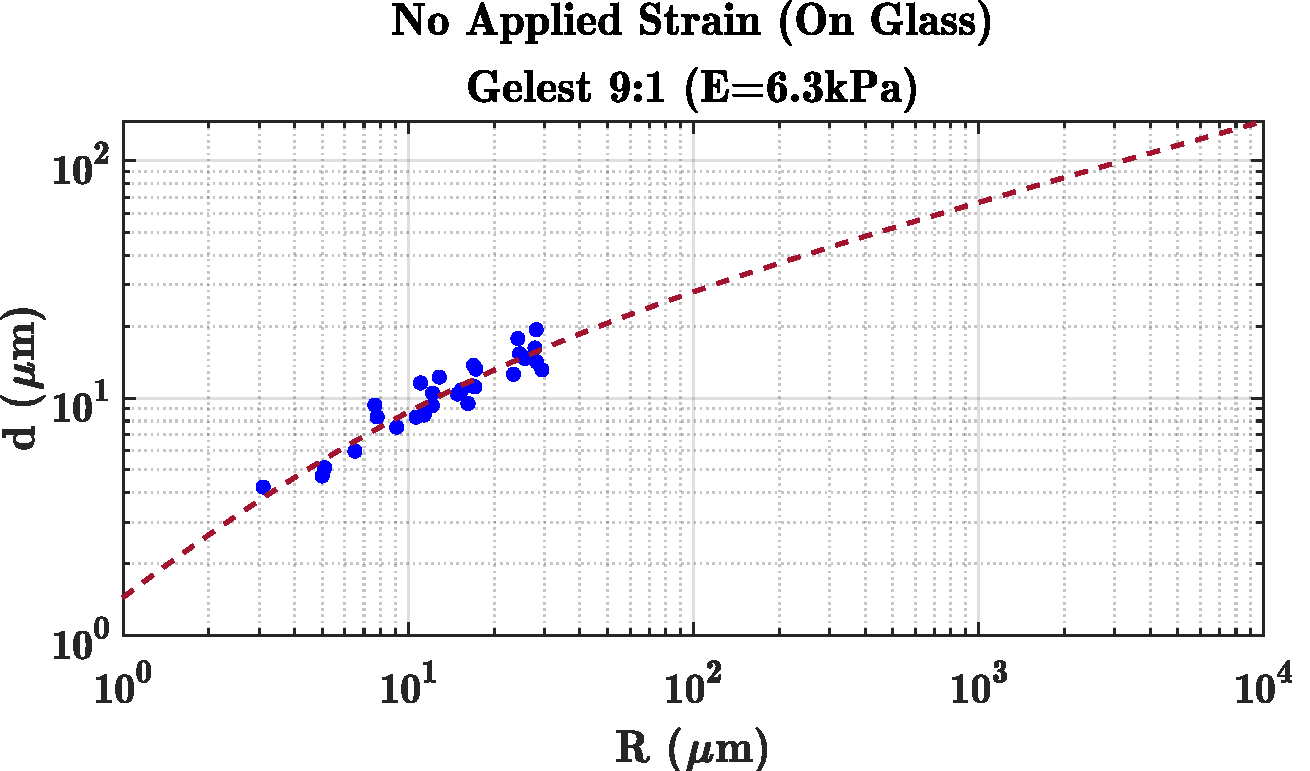
\includegraphics[width=\linewidth]{Chapters/Figures/w_ups_fit_G9-1}
	\caption[Gelest W-$\Upsilon$ Fit]{We fit Equation \ref{THEeqn} to the $ d $ vs.~$ R $ (depth vs. radius) plot for a Gelest 9:1 sample spun on glass. This is the same silicone sample as used in Figures \ref{fig:sc1unstretchedv8ml}--\ref{fig:glassvsstretched190218}. The best fit line returns parameters of $ W=53 $~mNm$^{-1}$  and $ \Upsilon=32 $~mNm$^{-1}$. These values agree well with previous measurements (see Table \ref{tab:upsilon_values}).}
	\label{fig:wupsfitg9-1}
\end{figure}

\section{Dow-Corning PDMS}
Because the first direct $ \Upsilon(\epsilon) $ measurement \cite{xu2017direct} was conducted using a Dow-Corning PDMS substrate, we are especially interested in using this material for our first $ \Upsilon(\epsilon) $ measurements. Since there has only been one measurement of $ \Upsilon(\epsilon) $ in soft matter, in order to have a value to use as comparison, we need to first use the same material. 

Our first measurements with Dow-Corning PDMS returned largely varying results; the stiffness of the silicone differed by a factor of 2 from the expected value, and the stiffness continued to increase as the silicone cured over a period of several weeks, as opposed to the usual 24 hour time-frame. Furthermore, the adhesion of the PDMS varied from sample to sample. Often the silica spheres would not adhere to the surface. It was eventually discovered that the Dow-Corning PDMS being used expired several years prior. Some of the measurements conducted, however, returned results of interest, and thus are included here.


\begin{figure}[h]
	\centering
	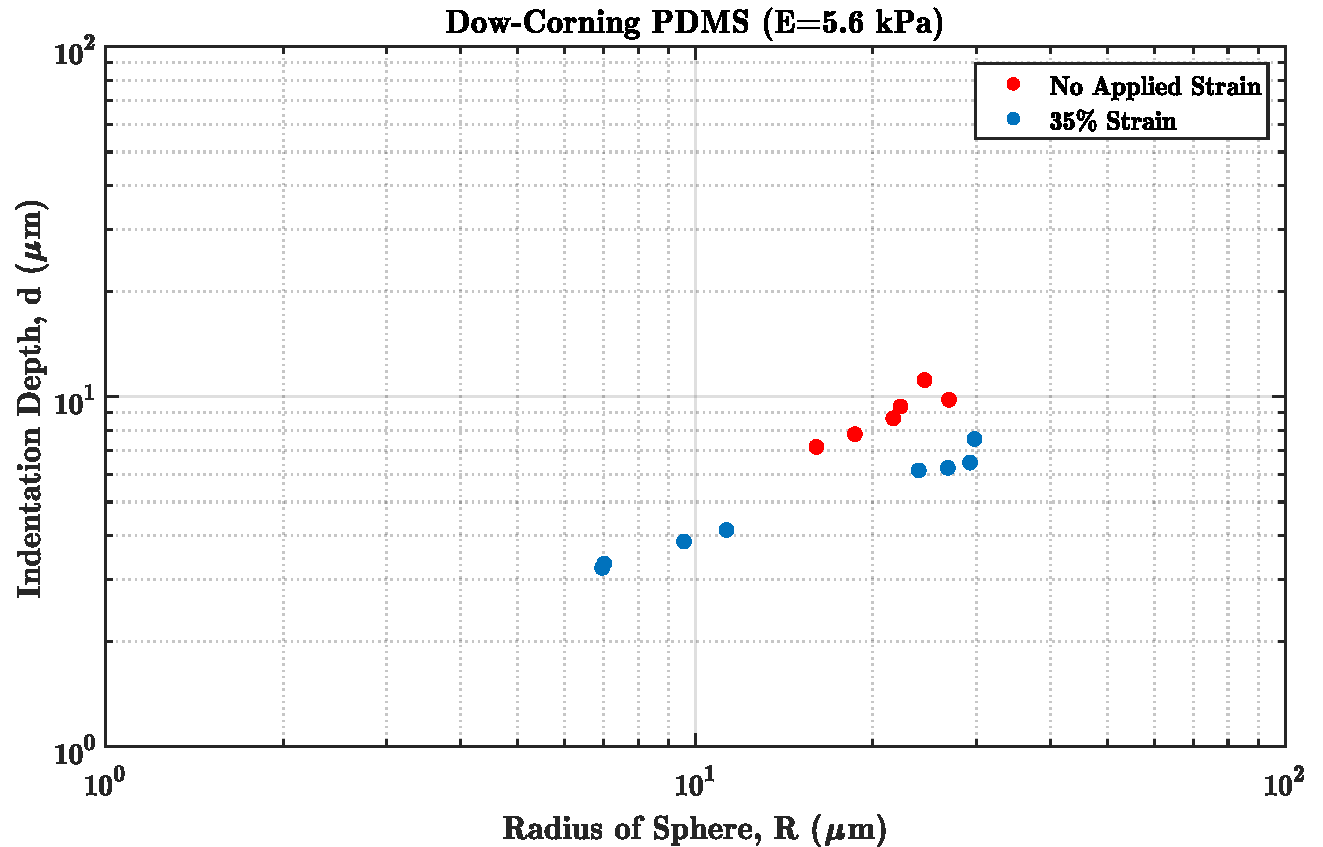
\includegraphics[width=\linewidth]{Chapters/Figures/d_vs_r_stretch_vs_nostretch.pdf}
	\caption[D vs. R Dow-Corning]{Plot of $ d $ vs.~$ R $ for a Dow-Corning [expired] PDMS substrate (191118) at two different strains. At higher strain, the spheres sink in less deep. This can be explained by an increase in $\Upsilon$ or an increase in $E$ for the substrate.}
	\label{fig:dvsrstretchvsnostretchdc181115}
\end{figure}

\begin{figure}[h]
	\centering
	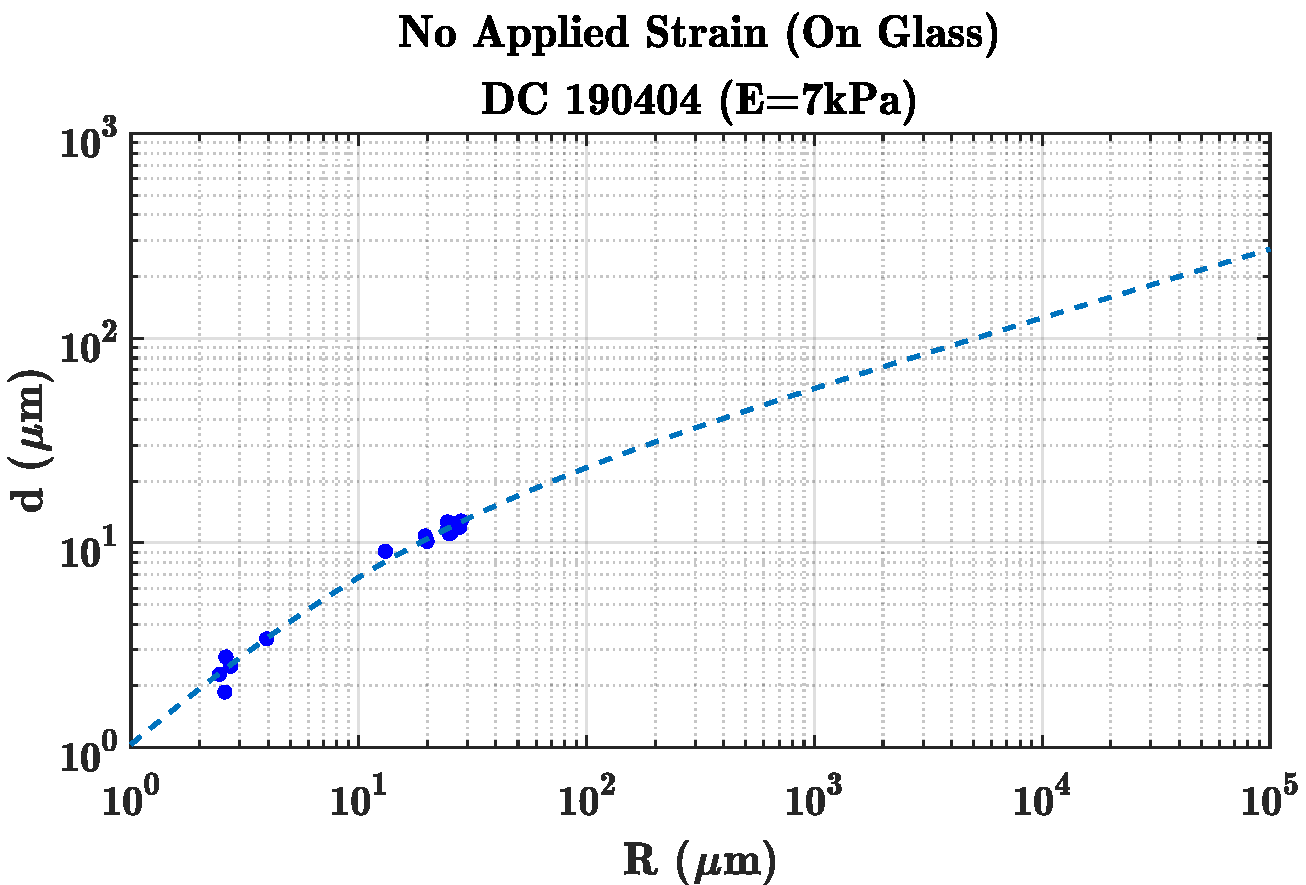
\includegraphics[width=\linewidth]{Chapters/Figures/WUps_fit_DC190404}
	\caption[Dow Corning W-$\Upsilon $ Fit]{The surface stress and adhesion energy fit for new Dow Corning PDMS silicone with no applied strain. Given the $ d $ vs.~$ R $ values, the fitting parameters to make the best fit line are W $ = 48.6$~mNm$^{-1}$ and  $\Upsilon = 43.5$ mNm$^{-1}$.}
	\label{fig:wupsfitdc190404}
\end{figure}

\section{Gelest and Dow-Corning PDMS Conclusions} \label{sec:DataConclusions}
Our $ d $ vs.~$ R $ data with the Gelest PDMS is clean for samples spun onto glass and returns reasonable values for $ \Upsilon $ and $ W $. Furthermore, we see a clear change in indentation depth for the individually tracked spheres (standard candles) under strain (Figure \ref{fig:sc1unstretchedv8ml}). Additionally, the average indentation depth for the strained sample compared to that spun onto glass is significantly shallower (Figure \ref{fig:glassvsstretched190218}). However, the $ d $ vs.~$ R $ data collected for Gelest on the stretching apparatus is noisy. As a consequence, we have yet to extract $ \Upsilon(\epsilon) $ and $ W(\epsilon) $. For Dow-Corning PDMS, our $ d $ vs.~$ R $ data with the new material is clean for samples spun onto glass, and returns reasonable values for $ \Upsilon $ and $ W $. As of the time writing, we have yet to test a stretchable sample of the new Dow-Corning PDMS.
\begin{figure}[h!]
	\centering
	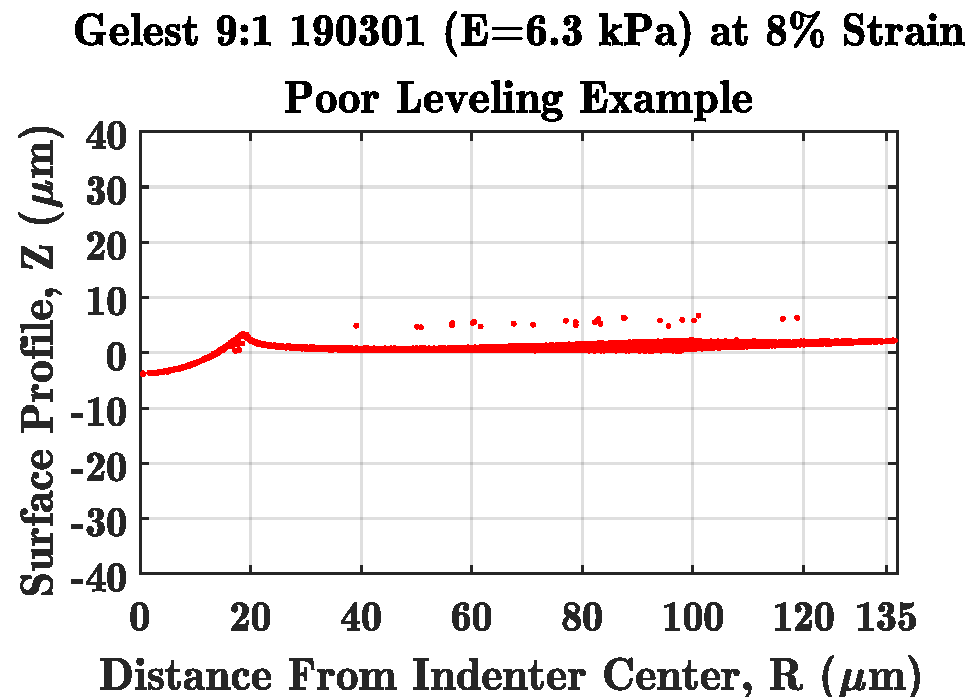
\includegraphics[width=.8\linewidth]{Chapters/Figures/190218G_tilted_axis_example}
	\caption[Side Collapse Tilt]{The side profile of a sphere on a stretched substrate. Notice how far away from the sphere, say $ R \approx 135 $, the surface is not at $ Z = 0 $, but instead a few microns above. For small tilts, such as those on a glass substrate, we can easily correct re-level the surface plane in using MATLAB software. However, the large tilts for the spheres collected on the stretching apparatus are problematic and not always correctable with software.}
	\label{fig:190218gtiltedaxisexample}
\end{figure}


Currently, the persistence of noise on our all $ d $ vs.~$ R $ data collected on the stretching apparatus is the main factor constraining our $ \Upsilon(\epsilon) $ and $ W(\epsilon) $ measurements. We hypothesize that the noise stems a large tilt found in all the data collected for substrates on the stretching apparatus. Upon close scrutiny of the azimuthally collapsed surface profile (e.g. Figure \ref{fig:sidecollapsed}) for spheres on stretchable substrates, many do not correctly ``zero'' the surface plane of the substrate. The surface profile is pulled up by the sphere due to adhesion, but returns to the surface plane far away from the sphere. However, for many of the spheres inspected, collapsing the side profile of the sphere caused the surface profile to be tilted away from zero far away from the sphere (See Figure \ref{fig:190218gtiltedaxisexample}). Conversely, leveling the profile has an adverse effect on the quality of the side collapse for the sphere. This tilt tends to be great enough such that the surface is between $ \pm 5~\mu$m at a distance of 140~$ \mu $m from the sphere. While this is only a tilt of $ 0.036 \degree $, it means that the depth measurements are off by 5~$ \mu $m, a significant discrepancy that would account for the noise.

Our MATLAB software attempts to correct for small tilts by leveling the surface plane of the located fluorescent beads, however, we suspect that this tilt my be too large to account for using our current software. Instead we have attempted to physically remove the tilt by leveling the stretching apparatus' mount. As of the date of writing, we have successfully leveled the mount, but have yet to collect data with this correction. 
